%%%%%%%%%%%%%%%%%%%%%%%%%%%%%%%%%%%%%%%%%
% Beamer Presentation
% LaTeX Template
% Version 1.0 (10/11/12)
%
% This template has been downloaded from:
% http://www.LaTeXTemplates.com
%
% License:
% CC BY-NC-SA 3.0 (http://creativecommons.org/licenses/by-nc-sa/3.0/)
%
%%%%%%%%%%%%%%%%%%%%%%%%%%%%%%%%%%%%%%%%%

%----------------------------------------------------------------------------------------
%	PACKAGES AND THEMES
%----------------------------------------------------------------------------------------

\documentclass{beamer}

\mode<presentation> {

% The Beamer class comes with a number of default slide themes
% which change the colors and layouts of slides. Below this is a list
% of all the themes, uncomment each in turn to see what they look like.

%\usetheme{default}
%\usetheme{AnnArbor}
%\usetheme{Antibes}
%\usetheme{Bergen}
%\usetheme{Berkeley}
%\usetheme{Berlin}
%\usetheme{Boadilla}
%\usetheme{CambridgeUS}
%\usetheme{Copenhagen}
%\usetheme{Darmstadt}
%\usetheme{Dresden}
%\usetheme{Frankfurt}
%\usetheme{Goettingen}
%\usetheme{Hannover}
%\usetheme{Ilmenau}
%\usetheme{JuanLesPins}
%\usetheme{Luebeck}
\usetheme{Madrid}
%\usetheme{Malmoe}
%\usetheme{Marburg}
%\usetheme{Montpellier}
%\usetheme{PaloAlto}
%\usetheme{Pittsburgh}
%\usetheme{Rochester}
%\usetheme{Singapore}
%\usetheme{Szeged}
%\usetheme{Warsaw}

% As well as themes, the Beamer class has a number of color themes
% for any slide theme. Uncomment each of these in turn to see how it
% changes the colors of your current slide theme.

%\usecolortheme{albatross}
%\usecolortheme{beaver}
%\usecolortheme{beetle}
%\usecolortheme{crane}
%\usecolortheme{dolphin}
%\usecolortheme{dove}
%\usecolortheme{fly}
%\usecolortheme{lily}
%\usecolortheme{orchid}
%\usecolortheme{rose}
%\usecolortheme{seagull}
%\usecolortheme{seahorse}
%\usecolortheme{whale}
%\usecolortheme{wolverine}

%\setbeamertemplate{footline} % To remove the footer line in all slides uncomment this line
%\setbeamertemplate{footline}[page number] % To replace the footer line in all slides with a simple slide count uncomment this line

%\setbeamertemplate{navigation symbols}{} % To remove the navigation symbols from the bottom of all slides uncomment this line
}
\setbeamertemplate{theorems}[numbered]

\usepackage{graphicx} % Allows including images
\usepackage{booktabs} % Allows the use of \toprule, \midrule and \bottomrule in tables
\usepackage{nicefrac}
\usepackage{xcolor}
\usepackage{wrapfig}
\usepackage{subcaption}
\usepackage[backend=biber, maxnames=10, uniquename=false, style=authoryear]{biblatex}
\bibliography{presentation_1.bib}
\usepackage{comment}

\definecolor{darkolivegreen}{rgb}{0.33, 0.42, 0.18}
\definecolor{ao_english}{rgb}{0.0, 0.5, 0.0}

%----------------------------------------------------------------------------------------
%	TITLE PAGE
%----------------------------------------------------------------------------------------

\title[Qual Presentation]{Qual Presentation} % The short title appears at the bottom of every slide, the full title is only on the title page

\author{Ziwei Ji} % Your name
\institute[UIUC] % Your institution as it will appear on the bottom of every slide, may be shorthand to save space
{
University of Illinois at Urbana-Champaign \\ % Your institution for the title page
\medskip
\textit{ziweiji2@illinois.edu} % Your email address
}
\date{\today} % Date, can be changed to a custom date

\begin{document}

\begin{frame}
\titlepage % Print the title page as the first slide
\end{frame}

\begin{frame}
\frametitle{Overview} % Table of contents slide, comment this block out to remove it
\tableofcontents % Throughout your presentation, if you choose to use \section{} and \subsection{} commands, these will automatically be printed on this slide as an overview of your presentation
\end{frame}

%----------------------------------------------------------------------------------------
%	PRESENTATION SLIDES
%----------------------------------------------------------------------------------------

%------------------------------------------------
\section{Self-Introduction}

\begin{frame}
\frametitle{About me}
\begin{itemize}
    \item Undergrad at Shanghai Jiaotong University.
    \item Worked with Prof. Ruta Mehta during my first year on algorithmic game theory.
    \item Switched to Prof. Matus Telgarsky last semester, working on machine learning theory.
\end{itemize}
\begin{itemize}
    \item I am interested in machine learning.
    \item I am interested in math, especially analysis.
\end{itemize}
\end{frame}

%------------------------------------------------

\section{Research}
\subsection{Loss and Parameter Convergence of Logistic Regression}
\begin{frame}
\frametitle{\phantom{}}
\Large Loss and Parameter Convergence of Logistic Regression
\end{frame}

\begin{frame}
\frametitle{Loss Convergence}
\onslide<2,3,4>{
Loss is convex, why not classical analysis?}

\onslide<3,4>{
\begin{itemize}
    \item The optimum is usually attained at the infinity.
    \begin{itemize}
        \item For example, the linearly separable case.
        \item See \cite{TDS15}, \cite{BFT17} for empirical results.
    \end{itemize}

    \item In classical analysis, existence of optimum usually assumed.
    \begin{itemize}
        \item Assuming smoothness and existence of optimum, $O(1/t)$ rate;
        \item Not assuming smoothness or existence of optimum, $O(1/\sqrt{t})$ rate.
    \end{itemize}
\end{itemize}}

\onslide<4>{
In this work, we
\begin{itemize}
    \item show an ${O}(\ln^2t/t)$ rate, even if optimum does not exist;
    \item show an implicit regularization property of gradient descent.
    \begin{itemize}
        \item If $w$ achieves lower loss than $w_t$, then $\|w\|>\|w_t\|/2$.
    \end{itemize}
\end{itemize}
}
\end{frame}

\begin{frame}
\frametitle{Parameter Convergence: In What Sense?}
\onslide<2,3>{
\begin{columns}[c]
\column{0.5\textwidth}
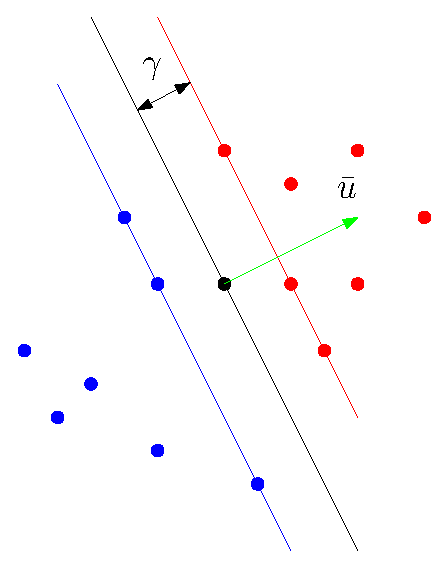
\includegraphics[width=0.8\textwidth]{separable.eps}
\column{0.5\textwidth}
Linearly separable case: {\color{red}$+1$, \color{blue}$-1$}.
\begin{itemize}
    \item $\bar{u}$: The normalized linear predictor with max margin.
    \item Normalized $w_t$ $\to$ $\bar{u}$.
    \item \onslide<3>{Why not SVM? Data points might not be linearly separable.}
\end{itemize}
\end{columns}}
\end{frame}

\begin{frame}
\frametitle{Parameter Convergence: In What Sense?}
\onslide<1>{
\begin{columns}[c]
\column{0.5\textwidth}
    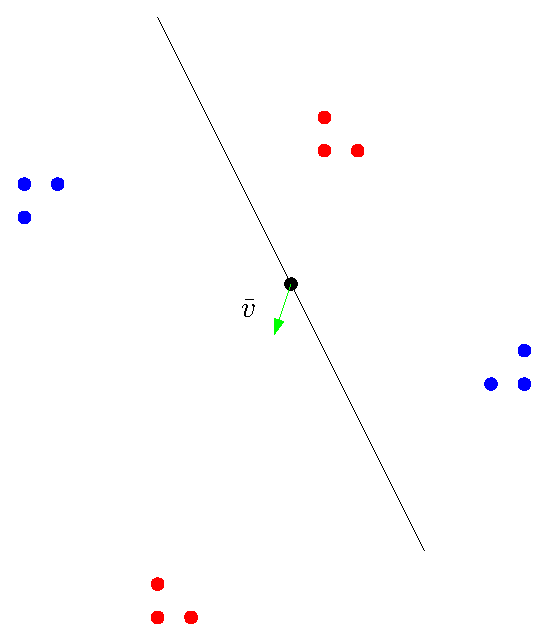
\includegraphics[width=0.8\textwidth]{strong_conv.eps}
\column{0.5\textwidth}
    Strongly convex case: {\color{red}$+1$, \color{blue}$-1$}.
    \begin{itemize}
        \item Strongly convex problem on sublevel set, Unique optimum solution $\bar{v}$.
        \item $w_t\to\bar{v}$.
    \end{itemize}
\end{columns}}
\end{frame}

\begin{frame}
\frametitle{Parameter Convergence: In What Sense?}
\onslide<1>{
\begin{columns}[c]
\column{0.5\textwidth}
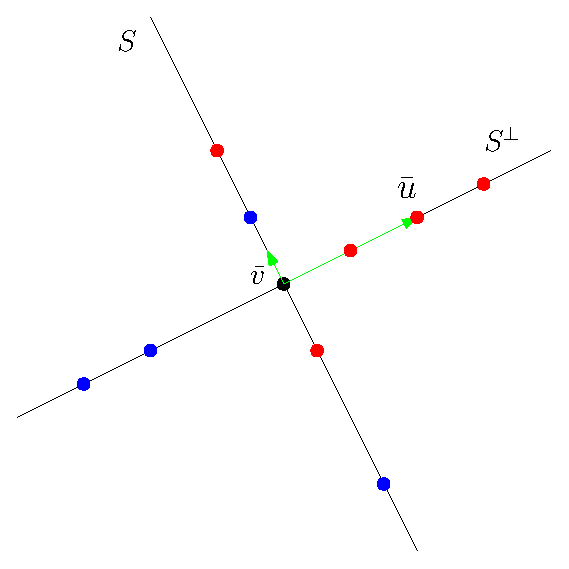
\includegraphics[width=0.8\textwidth]{simple_mixed.eps}
\column{0.5\textwidth}
A simple mixed case: {\color{red}$+1$, \color{blue}$-1$}.
\begin{itemize}
    \item Over $S$: Strongly convex, \newline unique $\bar{v}$.
    \item Over $S^{\perp}$: linearly separable, normalized $\bar{u}$ with max margin.
    \item GD progresses independently on $S$ and $S^{\perp}$:
    \begin{itemize}
        \item $\Pi_S(w_t)\to\bar{v}$;
        \item Normalized $\Pi_{S^{\perp}}(w_t)$ $\to$ $\bar{u}$.
    \end{itemize}
\end{itemize}
\end{columns}}
\end{frame}

\begin{frame}
\frametitle{Parameter Convergence: In What Sense?}
\onslide<1>{
\begin{columns}[c]
\column{0.5\textwidth}
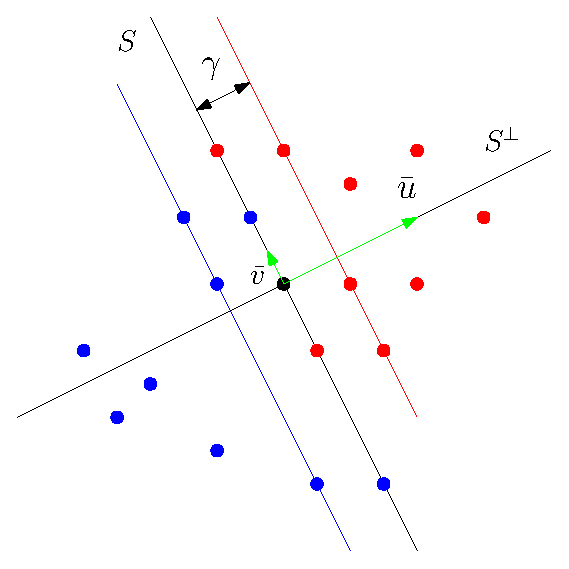
\includegraphics[width=0.8\textwidth]{mixed.eps}
\column{0.5\textwidth}
The general mixed case: {\color{red}$+1$, \color{blue}$-1$}.
\begin{itemize}
    \item $\bar{v}$ on $S$, $\bar{u}$ on $S^{\perp}$.
    \item GD on $S$ and $S^{\perp}$ are not independent! But still
    \begin{equation*}
        \left\|\Pi_S(w_t)-\bar{v}\right\|\le \tilde{O}\left(\frac{1}{t^{1/4}}\right),
    \end{equation*}
    and
    \begin{equation*}
        \left\|\frac{w_t}{\|w_t\|}-\bar{u}\right\|\le\tilde{O}\left(\frac{1}{\|w_t\|^{1/4}}\right).
    \end{equation*}
\end{itemize}
\end{columns}}
\end{frame}

\begin{frame}
\frametitle{Generalization Implications}
\begin{itemize}
    \item We have generalization bounds for strongly convex case and linearly separable case.
    \item In the mixed case, we can analyze $S$ and $S^{\perp}$ separately, and then get an overall generalization bound. See \cite{TDS15}.
\end{itemize}
\end{frame}

\begin{frame}
\frametitle{A Work in Parallel}
When data is linearly separable, we get a rate
\begin{equation*}
    \left\|\frac{w_t}{\|w_t\|}-\bar{u}\right\|\le\sqrt{\frac{\ln m+2}{\|w_t\|}}.
\end{equation*}

In parallel, \cite{SHS17} also considers separable data, and additionally exact $d$ support vectors with positive dual variables.
\begin{equation*}
    \left\|\frac{w_t}{\|w_t\|}-\bar{u}\right\|\le \frac{O(1)}{\|w_t\|}.
\end{equation*}
\end{frame}

\begin{frame}
\frametitle{Loss and Parameter Convergence of Logistic Regression}
\Large Questions?
\end{frame}

\subsection{Social Welfare Maximization from Revealed Preferences}
\begin{frame}
\frametitle{\phantom{}}
\Large Social Welfare Maximization from Revealed Preference
\end{frame}

\begin{frame}
\frametitle{Social Welfare Maximization from Revealed Preference}
\begin{itemize}
    \onslide<2,3,4,5>{\item Setting: Self-interested agents, maximize individual utilities:
    \begin{itemize}
        \item Consumers maximize (valuation - expenditure);
        \item Producers maximize (revenue - cost).
    \end{itemize}}
    \onslide<3,4,5>{\item Goal: Maximizing \emph{social welfare}: the sum of individual utilities, or (sum of valuation - sum of cost).}
    \onslide<4,5>{\item What to control: The prices.}
    \onslide<5>{\item How to learn good prices, what information do we have:
    \begin{itemize}
        \item Consumers' purchases (revealed preferences), and thus expenditures, are known;
        \item Consumers' true valuations are unknown (assumed to be known in classical work!)
    \end{itemize}}
\end{itemize}
\end{frame}

\begin{frame}
\frametitle{Difficulties and Solution}
\onslide<2,3>{
The social welfare is a non-concave function of prices.}

\vspace{10px}
\onslide<3>{
Solution:
\begin{itemize}
    \item The social welfare is concave of quantities of goods, while
    \newline
    prices are dual variables of a convex dual function.

    \item The optimum bundle of goods is induced by the optimum prices.

    \item The subgradient of the dual function comes from revealed preferences.
\end{itemize}
}
\end{frame}

\begin{frame}
\frametitle{Prior Work and This Work}
\onslide<1>{
\cite{RUW16} provides a two-layer optimization scheme:
\begin{itemize}
    \item An iterative algorithm $\mathcal{A}$ is run on the primal problem.
    \item For each step $\mathcal{A}$, a subroutine $\mathcal{B}$ is run on a dual problem.
\end{itemize}
The total running time is the product of running time of $\mathcal{A}$ and $\mathcal{B}$.
\begin{itemize}
    \item They proved $O(1/\epsilon^4)$.
    \item $O(1/\epsilon^3)$ is possible as far as I know.
\end{itemize}}

\onslide<1>{
\vspace{8px}
In our work, we
\begin{itemize}
    \item give $O(1/\epsilon^2)$ running time, by a direct optimization on the dual.;
    \item consider an online model, solved by online convex optimization methods.
\end{itemize}}
\end{frame}

\begin{frame}
\frametitle{Social Welfare Maximization from Revealed Preference}
\Large Questions?
\end{frame}

\subsection{Potential Future Research}
\begin{frame}
\frametitle{Potential Future Research}
Potential short term goals:
\begin{itemize}
    \item Wide application of optimization methods;
    \item NN generalization.
\end{itemize}

Potential long term goals:
\begin{itemize}
    \item SGD on NNs;
    \item Generalization, optimization, and representation of different models, such as RNN;
    \item Build strong relationships between theory and practice.
\end{itemize}
\end{frame}

%------------------------------------------------

\section{Paper Presentation}

%------------------------------------------------

\subsection{Size-Independent Sample Complexity of Neural Networks. Noah Golowich, Alexander Rakhlin, and Ohad Shamir, 2017.}
\begin{frame}
\frametitle{\phantom{}}
\Large Size-Independent Sample Complexity of Neural Networks. Noah Golowich, Alexander Rakhlin, and Ohad Shamir, 2017.
\end{frame}

\begin{frame}
\frametitle{Motivation}
\begin{itemize}
    \onslide<2,3,4,5>{\item Generalization: Low training error $\implies$ Low test error?}
    \onslide<3,4,5>{\item Classical Methods: VC dimension, Rademacher complexity; regularization; ...}
    \onslide<4,5>{\item \cite{ZBHRV16}: Empirically,\newline neural nets generalize well even if \# of params $>$ \# of data points.
    \begin{itemize}
        \item VC dimension seems to be helpless in this scenario.
    \end{itemize}}
    \item \onslide<5>{\cite{GRS17}: Generalization bounds which \newline do not depend on network size (i.e., depth and width) explicitly, but \newline on various weight matrices norms.}
\end{itemize}
\end{frame}

\begin{frame}
\frametitle{High-Level Idea}
\begin{itemize}
    \onslide<1>{\item Try to get some generalization bound with polynomial dependency on $d$ (and no explicit dependency on width).}
    \begin{itemize}
        \onslide<1>{\item One new result proved in this paper.}
        \onslide<1>{\item A result from \cite{BFT17} cited.}
    \end{itemize}
    \onslide<1>{\item Converting it into a depth-independent bound using a general framework.}
\end{itemize}
\end{frame}

\begin{frame}
\frametitle{Rademacher complexity}
\onslide<2,3>{
Given a data set $D$,
\begin{equation*}
    \mathcal{F}(D)=\left\{(f(x_1),\ldots,f(x_m))\middle|f\in \mathcal{F}\right\}
\end{equation*}}
\onslide<3>{
The Rademacher complexity of $\mathcal{F}(D)$ is defined as
\begin{equation*}
    \mathrm{Rad}\left(\mathcal{F}(D)\right)=\mathbb{E}_{\epsilon\sim U(\{-1,+1\}^m)}\left[\frac{1}{m}\sup_{f\in \mathcal{F}}\sum_{i=1}^{m}\epsilon_if(x_i)\right].
\end{equation*}
Intuitively, Rademacher complexity is the ability of $\mathcal{F}$ to fit random labels.
}
\end{frame}

\begin{comment}
\begin{frame}
\frametitle{From Rademacher to Generalization}
\begin{itemize}
    \onslide<2,3,4>{\item For any $f\in \mathcal{F}$, $x\in \mathcal{X}$, $f(x)\in[-R,+R]$.}
    \onslide<3,4>{\item $\ell$ is $\lambda$-Lipschitz.}
\end{itemize}
\onslide<4>{
With probability at least $1-\delta$ over $D$,
\begin{equation*}
    \sup_{f\in \mathcal{F}}\left(R(f)-R_D(f)\right)\le \frac{2\lambda}{m}\mathrm{Rad}\left(\mathcal{F}(D)\right)+6\lambda R\sqrt{\frac{\ln(2/\delta)}{2m}}.
\end{equation*}
}
\end{frame}

\begin{frame}
\frametitle{Linear Predictors}
\begin{itemize}
    \item \onslide<2,3,4,5>{$\|x\|\le M$.}
    \item \onslide<3,4,5>{Linear predictors $\|w\|\le B$.}
    \item \onslide<4,5>{Then $\mathrm{Rad}(\mathcal{F}_{\mathrm{lin}}(D))\le MB\sqrt{m}$.}
    \item \onslide<5>{Unbounded linear predictors? Post hoc guanratees.}
\end{itemize}
\end{frame}
\end{comment}

\begin{frame}
\frametitle{From Rademacher to Generalization}
\onslide<2,3,4>{
\begin{equation*}
    \mathcal{F}_d=\{\sigma_d(W_d\sigma_{d-1}(W_{d-1}\cdots\sigma_1(W_1x)))\}.
\end{equation*}
$\sigma_1,\ldots,\sigma_d$ are identity or ReLU.}

\onslide<3,4>{Lipschitz-style assumptions: Loss function is Lipschitz, $\|x\|\le1$, $\|W_j\|\le M(j)$.}

\onslide<4>{
With high probability,
\begin{equation*}
    \colorlet{oldcolor}{.}
    \textrm{test error}-\textrm{training error}\le O\left(\mathrm{Rad}\left(\mathcal{F}_d(D)\right)+\prod_{j=1}^{d}{M(j)}\sqrt{\frac{1}{m}}\right).
\end{equation*}
%\quad\quad\quad\quad\quad\quad\quad\quad\quad\quad\quad\quad\quad\quad\quad{\color{blue}complexity error}\quad{\color{ao_english}concentration error}
}
\end{frame}

\begin{frame}
\frametitle{A Negative Result}
\begin{itemize}
    \onslide<2,3,4>{\item Ideally,
    \begin{equation*}
        \mathrm{Rad}\left(\mathcal{F}_d(D)\right)\le C\cdot \prod_{j=1}^{d}M(j)\cdot \frac{1}{\sqrt{m}}.
    \end{equation*}
    }
    \onslide<3,4>{\item However, Theorem 7 of \cite{GRS17} shows that a dependency on network width is unavoidable.}
    \onslide<4>{\item Size-independent? More assumptions are made: $\prod\|W_j\|\ge\ldots$, $\|W_j\|_p\le\ldots$ ($p<\infty$).}
\end{itemize}
\end{frame}

\begin{frame}
\frametitle{Size-Independent Sample Complexity of Neural Networks}
\Large Any questions before bounds of the paper?
\end{frame}

\begin{frame}
\frametitle{High-Level Idea (A Two-Step Approach)}
\begin{itemize}
    \onslide<1>{\item Try to get some generalization bound with polynomial dependency on $d$ (and no explicit dependency on width).}
    \begin{itemize}
        \onslide<1>{\item One new result proved in this paper.}
        \onslide<1>{\item A result from \cite{BFT17} cited.}
    \end{itemize}
    \onslide<1>{\item Converting it into a depth-independent bound using a general framework.}
\end{itemize}
\end{frame}

\begin{frame}
\frametitle{Exp-Depth Frobenius Bound}
\onslide<1,2>{
\begin{align*}
    \colorlet{oldcolor}{.}
    mRad(\mathcal{F}_d(D)) & =\mathbb{E}_{\epsilon}\left[\sup_{f\in \mathcal{F}_d}\sum_{i=1}^{m}\epsilon f(x_i)\right] \\
     & \le{\color{blue}\boxed{\color{black}\mathbb{E}_{\epsilon}\left[\sup_{f\in \mathcal{F}_d}\left|\sum_{i=1}^{m}\epsilon f(x_i)\right|\right]}\quad(d-\textrm{layer complexity})} \\
     & \le 2M_F(d)\cdot{\color{blue}\boxed{\color{black}\mathbb{E}_{\epsilon}\left[\sup_{f\in \mathcal{F}_{d-1}}\left\|\sum_{i=1}^{m}\epsilon f(x_i)\right\|\right]}},
\end{align*}
\quad\quad\quad\quad\quad\quad\quad\quad\quad\quad\quad\quad\quad\ {\color{blue}$(d-1)$-layer complexity}

where $\|W_d\|_F\le M_F(d)$.}

\onslide<2>{
{\color{red}2 is accumulated multiplicatively!}}
\end{frame}

\begin{frame}
\frametitle{Poly-Depth Frobenius Bound}
\onslide<1,2>{
\begin{align*}
    mRad(\mathcal{F}_d(D)) & =\mathbb{E}_{\epsilon}\left[\sup_{f\in \mathcal{F}_d}\sum_{i=1}^{m}\epsilon f(x_i)\right] \\
     & \le \mathbb{E}_{\epsilon}\left[\sup_{f\in \mathcal{F}_d}\left|\sum_{i=1}^{m}\epsilon f(x_i)\right|\right] \\
     & \le \frac{1}{\lambda}\ln{\color{blue}\boxed{\color{black}\mathbb{E}_{\epsilon}\left[\sup_{f\in \mathcal{F}_d}\exp\left(\lambda\left|\sum_{i=1}^{m}\epsilon f(x_i)\right|\right)\right]}\quad d\textrm{-layer complexity}} \\
     & \le \frac{1}{\lambda}\ln\left(2{\color{blue}\boxed{\color{black}\mathbb{E}_{\epsilon}\left[\sup_{f\in \mathcal{F}_{d-1}}\exp\left(M_F(d)\cdot\lambda\left\|\sum_{i=1}^{m}\epsilon f(x_i)\right\|\right)\right]}}\right).
\end{align*}
\quad\quad\quad\quad\quad\quad\quad\quad\quad\quad\quad\quad\quad\quad\quad{\color{blue}$(d-1)$-layer complexity}}

\onslide<2>{
{\color{red}2 is accumulated multiplicatively in $\ln$!}
}
\end{frame}

\begin{frame}
\frametitle{Poly-Depth Frobenius Bound}
\begin{theorem}[\cite{GRS17} Theorem 1]
\begin{equation*}
    \mathrm{Rad}(\mathcal{F}_d(D))\le O\left(\prod_{j=1}^{d}M_F(j)(\sqrt{2\ln(2)d}+1)\cdot \frac{1}{\sqrt{m}}\right).
\end{equation*}
\end{theorem}
\end{frame}

\begin{frame}
\frametitle{From Size-Dependent to Size-Independent}
\onslide<2,3>{
\begin{align*}
    \mathcal{F}_d\ni f & \xrightarrow[\text{or 0}]{\text{replace $W_r$ with its rank-1 approx}}\tilde{f}\in\tilde{\mathcal{F}}_{d,r} \\
\end{align*}}
\onslide<3>{
\begin{equation*}
    \mathrm{Rad}[\mathcal{F}_d(D)]\le{\color{blue}\boxed{\color{black}\mathrm{Rad}(\tilde{\mathcal{F}}_{d,r}(D))}}+{\color{ao_english}\boxed{\color{black}\sup_{x,f}|f(x)-\tilde{f}(x)|}}.
\end{equation*}
\quad\quad\quad\quad\quad\quad\quad\quad\quad\quad\quad\quad$\le O(r^{\alpha})$\quad\quad\quad\quad$\le O(r^{-\beta})$
\begin{itemize}
    \item Balance the above two terms, and get a bound independent of $r$ or $d$.
\end{itemize}
}
\end{frame}

\begin{frame}
\frametitle{$\mathrm{Rad}(\tilde{\mathcal{F}}_{d,r}(D))\le O(r^{\alpha})$}
\begin{itemize}
    \onslide<2,3>{
    \item For each $\tilde{f}\in\tilde{\mathcal{F}}_{d,r}$, the $r$-th layer of $\tilde{f}$ is of rank at most 1.
    \item With this property and Theorem 4 in \cite{GRS17},
    \begin{equation*}
        \mathrm{Rad}(\tilde{\mathcal{F}}_{d,r}(D))\le\tilde{O}\left({\color{blue}\boxed{\color{black}\prod_{j=1}^{d}M(j)\cdot \frac{1}{\sqrt{m}}}}+{\color{ao_english}\boxed{\color{black}\prod_{j=r+1}^{d}M(j)\cdot Rad(\mathcal{F}_r(D))}}\right).
    \end{equation*}
    \quad\quad\quad\quad\quad\quad\quad\quad\quad\ \ {\color{blue}$r$-independent}\quad\quad\quad\ {\color{ao_english}poly-$r$ dependency}
    }
    \onslide<3>{\item If we plug in the Frobenius norm bound, we get
    \begin{equation*}
        \mathrm{Rad}(\tilde{\mathcal{F}}_{d,r}(D))\le\tilde{O}\left(\prod_{j=1}^{d}M_F(j)\cdot \frac{1}{\sqrt{m}}\cdot\sqrt{r}\right).
    \end{equation*}}

\end{itemize}
\end{frame}

\begin{comment}
\begin{frame}
\frametitle{$\mathrm{Rad}(\tilde{\mathcal{F}}_{d,r}(D))\le O(r^{\alpha})$}
\onslide<2,3>{
\begin{equation*}
    \tilde{f}(\mathbf{x})=\sigma_d(W_d\cdots\sigma_{r}(s \mathbf{u}\mathbf{v}^{\top}\cdots\sigma_1(W_1 \mathbf{x}))),
\end{equation*}
}
\onslide<3>{
which is a depth-$r$ neural net
\begin{equation*}
    \mathbf{x}\mapsto s \mathbf{v}^{\top}\sigma_{r-1}(W_{r-1}\cdots\sigma_1(W_1 \mathbf{x}))
\end{equation*}
composed with a univariate Lipschitz function (mapping $0$ to $0$)
\begin{equation*}
    t\mapsto\sigma_d(W_d\cdots \mathbf{u}t).
\end{equation*}
}
\end{frame}

\begin{frame}
\frametitle{$\mathrm{Rad}(\tilde{\mathcal{F}}_{d,r}(D))\le O(r^{\alpha})$}
\cite{GRS17} Theorem 4 allows us to show that
\begin{equation*}
    \mathrm{Rad}(\tilde{\mathcal{F}}_{d,r}(D))\le \prod_{j=1}^{d}M(j)\cdot \tilde{O}\left({\color{blue}\boxed{\color{black}\sqrt{m}}}+{\color{ao_english}\boxed{\color{black}\frac{Rad(\mathcal{F}_r(D))}{\prod_{j=1}^{r}M(j)}}}\right).
\end{equation*}
\quad\quad\quad\quad\quad\quad\quad\quad\quad\quad\quad\quad\quad\quad\quad{\color{blue}depth-indep}\quad\ {\color{ao_english}poly-depth}
\end{frame}
\end{comment}

\begin{frame}
\frametitle{Approximation Error $\le O(r^{-\beta})$}
\begin{itemize}
    \onslide<2,3>{\item $|f(x)-\tilde{f}(x)|$ depends on $\|W_r\|_p/\|W_r\|$; want it to be small. How?}
    \onslide<3>{\item Assume $\prod_{j=1}^{d}\|W_j\|_p/\|W_j\|\le Z$.
    \item Under this assumption, {\color{red}there exists} $1\le d\le r$,
    \begin{equation*}
        \|W_d\|_p/\|W_d\|\le Z^{1/r},
    \end{equation*}
    and if we replace $W_d$,
    \begin{equation*}
        \sup_{\|x\|\le1}|f(x)-\tilde{f}(x)|\le O\left(\prod_{j=1}^{d}\|W_j\|\left(\frac{\ln Z}{r}\right)^{1/p}\right).
    \end{equation*}
    }
\end{itemize}
\end{frame}

\begin{frame}
\frametitle{Proof Idea Review}
\onslide<1,2>{
\begin{equation*}
    \mathcal{F}_d\ni f \rightarrow\tilde{f}\in\tilde{\mathcal{F}}
\end{equation*}
\\
\begin{equation*}
    \mathrm{Rad}[\mathcal{F}_d(D)]\le\mathrm{Rad}(\tilde{\mathcal{F}}(D))+\sup_{x,f}|f(x)-\tilde{f}(x)|.
\end{equation*}}
\\
\onslide<2>{
\begin{equation*}
    \mathrm{Rad}[\mathcal{F}_d(D)]\le{\color{blue}\boxed{\color{black}\mathrm{Rad}\left({\color{red}\bigcup_{e=1}^r\tilde{\mathcal{F}}_{d,e}(D)}\right)}}+{\color{ao_english}\boxed{\color{black}m\sup_{x}|f(x)-\tilde{f}(x)|}}.
\end{equation*}
\quad\quad\quad\quad\quad\quad\quad\quad\quad\quad\quad$\le O(r^{\color{red}\alpha+1})$\quad\quad\quad$\le O(r^{-\beta})$
}
\end{frame}

\begin{frame}
\frametitle{A Frobenius Norm Bound}
They claim
\begin{equation*}
    Rad(\mathcal{F}_d(D))\le\tilde{O}\left(\prod_{j=1}^{d}M_F(j)\cdot m^{-1/4}\right).
\end{equation*}
{\color{red}With the fix}, we get
\begin{equation*}
    Rad(\mathcal{F}_d(D))\le\tilde{O}\left(\prod_{j=1}^{d}M_F(j)\cdot m^{\color{red}-1/8}\right).
\end{equation*}
\end{frame}

\begin{frame}
\frametitle{Discussion}
\begin{itemize}
    \item Even if $\|W\|$ is bounded, $\|W\|_F$ can be as large as $\sqrt{h}\|W\|$, where $h$ is the width of the network.

    They also cite a bound from \cite{BFT17}, but they assume $\|W_j^T\|_{2,1}/\|W_j\|\ge \|W_j\|_F/\|W_j\|$ is bounded.
    \item Empirical results?
\end{itemize}
\end{frame}

\begin{frame}
\frametitle{Conclusion}
\begin{itemize}
    \item A generalization bound depending on $\prod_{j=1}^{d}M_F(j)$ and $\sqrt{d}$.
    \item A general framework for converting a depth-dependent bound to a depth-independent one.
\end{itemize}
\end{frame}

%------------------------------------------------

\begin{frame}
\frametitle{References}
\printbibliography
\end{frame}

%------------------------------------------------

\begin{frame}
\Large{\centerline{Thanks!}}
\end{frame}

%----------------------------------------------------------------------------------------

\end{document}

\begin{comment}
\begin{frame}
\frametitle{Formal Description}
\begin{itemize}
    \onslide<1>{\item $d$ divisible goods.}
    \onslide<1>{\item $1$ consumer (wlog), concave valuation $v:\mathbb{R}_+^d\to \mathbb{R}_+$, unknown.}
    \onslide<1>{\item $1$ producer, convex cost $c:\mathbb{R}_+^d\to \mathbb{R}_+$, known.
    \begin{itemize}
        \item The producer produces whatever the consumers demands.
    \end{itemize}}
    \onslide<1>{\item Given prices $p\in \mathbb{R}_+^d$, the consumer buys a "utility-maximizing bundle"
    \begin{equation*}
        x(p)\in\arg\max\left(v(x)-\langle x,p\rangle\right).
    \end{equation*}}
    \onslide<1>{\item Social welfare, (valuation - cost).
    \begin{equation*}
        v\left(x(p)\right)-c\left(x(p)\right).
    \end{equation*}}
\end{itemize}
\end{frame}

\begin{frame}
\frametitle{Formal Description}
\onslide<1>{How to maximize $v\left(x(p)\right)-c\left(x(p)\right)$ with $x(p)$?}

\onslide<1>{Two observations:}
\begin{itemize}
    \onslide<1>{\item By Fenchel duality,
    \begin{equation*}
        \sup\left(v(x)-c(x)\right)=\inf\left(c^*(p)-v^*(p)\right).
    \end{equation*}}

    \onslide<1>{\item By definition of conjugacy,
    \begin{equation*}
        x(p)\in\arg\max\left(v(x)-\langle x,p\rangle\right)\iff x(p)\in\partial v^*(p).
    \end{equation*}}
\end{itemize}
\end{frame}
\end{comment}

\begin{comment}
\begin{frame}
\frametitle{Loss and Parameter Convergence of Logistic Regression}
\begin{itemize}
    \onslide<2,3,4>{\item $(x_1,y_1),\ldots,(x_m,y_m)$, where $x_i\in \mathbb{R}^d$, $\|x_i\|\le1$, and $y_i\in\{-1,+1\}$.}
    \onslide<3,4>{\item Learn a linear predictor $w\in \mathbb{R}^d$; unconstrained optimization.}
    \onslide<4>{\item Given $\ell$ ($\ell_{\mathrm{exp}}(z)=\exp(z)$ or $\ell_{\mathrm{log}}(z)=\ln\left(1+\exp(z)\right)$ in this work), minimize
    \begin{equation*}
        R_m(w)=\sum_{i=1}^{m}\ell\left(-y_i \langle w,x_i\rangle\right).
    \end{equation*}}
\end{itemize}
\end{frame}

\begin{frame}
\frametitle{No Optimum Solution}
\begin{itemize}
    \onslide<2,3,4>{\item For example, if $m=1$, $x_1=y_1=+1$.}
    \onslide<3,4>{\item In smooth optimization, the existence of optimum solution was always assumed.}
    \onslide<4>{\item Smooth condition can give better convergence rate.}
\end{itemize}
\end{frame}

\begin{frame}
\frametitle{Loss Convergence}
\onslide<2,3,4>{
\begin{theorem}
    Let $w_0=0$, and $w_{t+1}=w_t-\eta_t\nabla R_m(w_t)$ such that $\eta_t\le1$. Then for $\ell_{\mathrm{exp}}$ or $\ell_{\mathrm{log}}$, any $t\ge1$ and $w\in \mathbb{R}^d$,
    \begin{equation*}
        R_m(w_t)-R_m(w)\le \frac{\|w\|^2-\|w_t-w\|^2}{2 \sum_{i=0}^{t-1}\eta_i}.
    \end{equation*}
\end{theorem}
}
\only<3>{
\begin{corollary}
    In separable case, let $w=\bar{u}\ln t/\gamma$, $\eta_t=1$, then
    \begin{equation*}
        R_m(w_t)\le \frac{1}{t}+\frac{\ln^2t}{2t}.
    \end{equation*}
\end{corollary}
}
\only<4>{
\begin{corollary}[Implicit Regularization]
    For any $t\ge1$, any $w\in \mathbb{R}^d$, if $\|w_t\|\ge2\|w\|$, then $R_m(w_t)\le R_m(w)$. In other words, if $R_m(w)<R_m(w_t)$, then $\|w_t\|<2\|w\|$.
\end{corollary}
}
\end{frame}

\begin{frame}
\frametitle{Parameter Convergence}
\onslide<2,3>{
\begin{theorem}
    Under the same condition, for $\ell_{\mathrm{exp}}$,
    \begin{equation*}
        \left\|\frac{w_t}{\|w_t\|}-\bar{u}\right\|^2\le \frac{\ln m+2}{\|w_t\|}.
    \end{equation*}
\end{theorem}
}
\onslide<3>{
Working on better convergence rate for $\ell_{\mathrm{log}}$.
}
\end{frame}

\begin{frame}
\frametitle{Related Work}
In parallel, \cite{SHS17} also considers parameter convergence for separable data.
\begin{itemize}
    \item Assume there are exactly $d$ support vectors, whose dual variables are positive, they show that
    \begin{equation*}
        \left\|\frac{w_t}{\|w_t\|}-\bar{u}\right\|^2\le \frac{O(1)}{\|w_t\|^2}.
    \end{equation*}

    \item They do not consider the non-separable case.
\end{itemize}
\end{frame}

\begin{frame}
\frametitle{Non-separable case}
\onslide<2,3,4,5>{
{\color{red}$+1$}, {\color{blue}$-1$}.
\begin{figure}
    \centering
    \begin{subfigure}[b]{0.3\textwidth}
        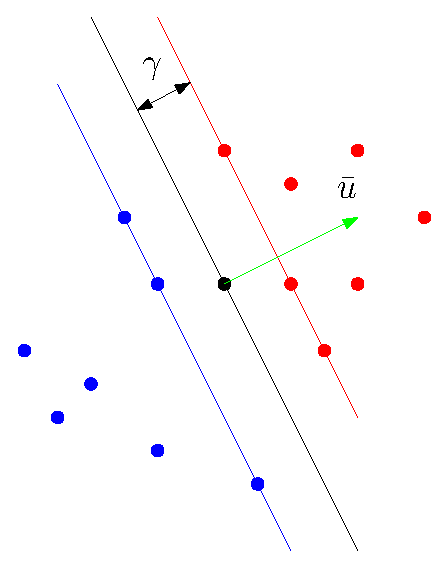
\includegraphics[width=0.8\textwidth]{separable.eps}
        \caption{Separable Case.}
    \end{subfigure}
    \quad
    \begin{subfigure}[b]{0.3\textwidth}
        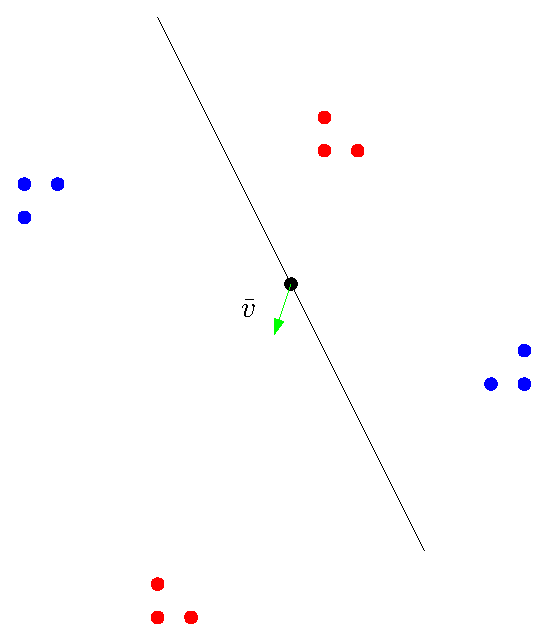
\includegraphics[width=\textwidth]{strong_conv.eps}
        \caption{Strongly Convex Case.}
    \end{subfigure}
    \quad
    \begin{subfigure}[b]{0.3\textwidth}
        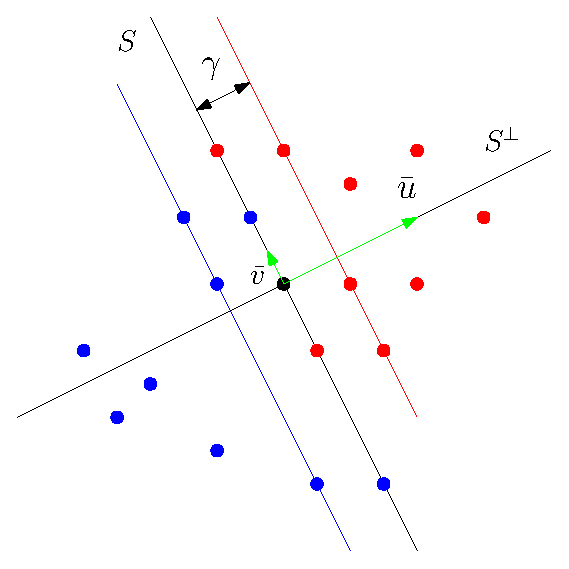
\includegraphics[width=\textwidth]{mixed.eps}
        \caption{Mixed Case.}
    \end{subfigure}
\end{figure}
}
\only<3>{
(a): Loss infimum equals 0; no optimum solution.
}
\only<4>{
(b): Loss minimum larger than 0; optimum solution $\bar{v}$.
}
\only<5>{
(c): Loss infimum larger than 0; no optimum solution.
}
\end{frame}

\begin{frame}
\frametitle{Loss Convergence}
\onslide<2,3,4>{
\begin{theorem}
    Let $w_0=0$, and $w_{t+1}=w_t-\eta_t\nabla R_m(w_t)$ such that $\eta_t\le1$. Then for $\ell_{\mathrm{exp}}$ or $\ell_{\mathrm{log}}$, any $t\ge1$ and $w\in \mathbb{R}^d$,
    \begin{equation*}
        R_m(w_t)-R_m(w)\le \frac{\|w\|^2-\|w_t-w\|^2}{2 \sum_{i=0}^{t-1}\eta_i}.
    \end{equation*}
\end{theorem}
}
\only<3>{
\begin{corollary}
    In separable case, let $w=\bar{v}+\nicefrac{\bar{u}\ln t}{\gamma}$, $\eta_t=1$, then
    \begin{equation*}
        R_m(w_t)-\inf_{w\in \mathbb{R}^d}R_m(w)\le \frac{\exp(2\|\bar{v}\|)}{t}+\frac{\ln^2t}{2t}.
    \end{equation*}
\end{corollary}
}
\only<4>{
\begin{corollary}
    In separable case, let $w=\bar{v}+\nicefrac{\bar{u}\ln t}{\gamma}$, $\eta_t=1/\sqrt{t+1}$, then
    \begin{equation*}
        R_m(w_t)-\inf_{w\in \mathbb{R}^d}R_m(w)\le \frac{\exp(2\|\bar{v}\|)}{t}+\frac{\ln^2t}{\sqrt{t}}.
    \end{equation*}
\end{corollary}
}
\end{frame}

\begin{frame}
\frametitle{Parameter Convergence}
\onslide<2,3>{
\begin{theorem}
    Under the same condition, for $\ell_{\mathrm{exp}}$,
    \begin{equation*}
        \left\|\frac{w_t}{\|w_t\|}-\bar{u}\right\|^2\le \tilde{O}\left(\frac{1}{\sqrt{\|w_t\|}}\right).
    \end{equation*}
\end{theorem}
}
\onslide<3>{
Working on better convergence rate for $\ell_{\mathrm{log}}$.
}
\end{frame}

\begin{frame}
\frametitle{Generalization Error}
\begin{itemize}
    \onslide<1>{
    \item Given $D$, our algorithm output $f_D\in \mathcal{F}$.
    \item $R(f)$: True risk, (roughly) test error.
    \newline $R_D(f)$: Empirical risk, training error.
    }
    \onslide<1>{
    \item Generalization error:
    \begin{equation*}
        R(f_D)-R_D(f_D).
    \end{equation*}
    }
    \onslide<1>{
    \item Uniform deviation:
    \begin{equation*}
        {\color{red}\boxed{\color{black}U_D(\mathcal{F})}}=\sup_{f\in \mathcal{F}}\left(R(f)-R_D(f)\right).
    \end{equation*}
    \quad\quad\quad\quad\quad\quad\quad\ \ {\color{red}takeaway}
    }
\end{itemize}
\end{frame}
\end{comment}

\begin{comment}
\begin{frame}
\frametitle{Original Plan}
\begin{equation*}
    \mathrm{Rad}[\mathcal{F}_d(D)]\le{\color{blue}\boxed{\color{black}\mathrm{Rad}(\tilde{\mathcal{F}}_{d,r}(D))}}+{\color{ao_english}\boxed{\color{black}m\sup_{x}|f(x)-\tilde{f}(x)|}}.
\end{equation*}
\quad\quad\quad\quad\quad\quad\quad\quad\quad\quad\quad$\le O(r^{\alpha}\cdot\sqrt{m})$\quad\quad\quad$\le O(r^{-\beta}\cdot m)$
\end{frame}

\begin{frame}
\frametitle{Bug Fix}
\begin{equation*}
    \mathrm{Rad}[\mathcal{F}_d(D)]\le{\color{blue}\boxed{\color{black}\mathrm{Rad}\left({\color{red}\bigcup_{e=1}^r\tilde{\mathcal{F}}_{d,e}(D)}\right)}}+{\color{ao_english}\boxed{\color{black}m\sup_{x}|f(x)-\tilde{f}(x)|}}.
\end{equation*}
\quad\quad\quad\quad\quad\quad\quad\quad\quad\quad\quad$\le O(r^{\color{red}\alpha+1}\cdot\sqrt{m})$\quad\quad\quad$\le O(r^{-\beta}\cdot m)$
\end{frame}
\end{comment}
